\section[Exceptions in Java]{Exceptions in Java}
Java中的异常分为两类:checked exception和runtime exception(uncheck exception),
如图\ref{fig:exceptions}所示,
RuntimeException及其子类叫做runtime exception,也叫做uncheck exception,
Exception的其他子类叫做checked exception。

\begin{figure}
  \centering
  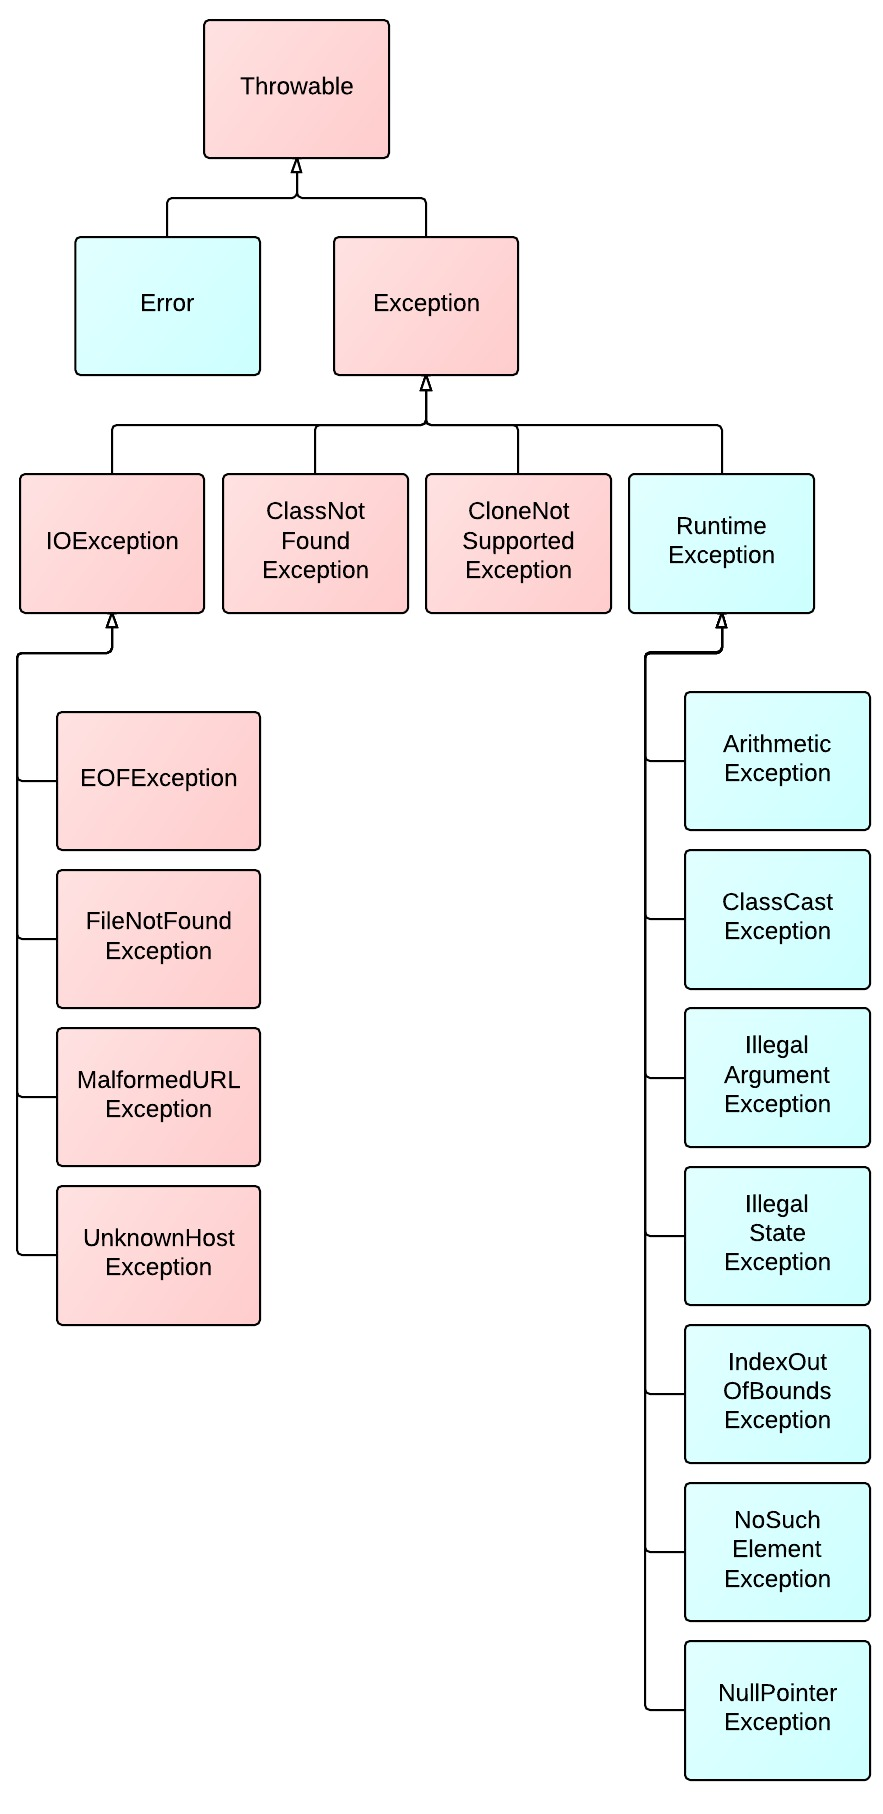
\includegraphics[width=0.7\textwidth]{picturedir/JavaExceptions.jpeg}\\
  \caption{Java的异常体系}\label{fig:exceptions}
\end{figure}

\subsection[名字的由来]{名字的由来}
所谓的checked与uncheck指的是compiler的行为,即compiler在编译时(废话,肯定是编译时)
作检查(check)的exception叫做checked exception,其他exception叫做runtime exception,
也叫做uncheck exception,

\begin{javacode}
class ExceptionTest {
  void testCheckedException() throws IOException { }
  void testRuntimeException() throws IndexOutOfBoundsException { }
  void test() {
    testCheckedException(); // compile error
    testRuntimeException(); // no compile error
  }
}
\end{javacode}

\subsection[设计的初衷]{设计的初衷}
在一个方法的实现者角度来看,checked exception意味着我知道在该方法被调用的过程中
可能会发生某些异常,但是对此我无能为力,我只能throws exception(方法签名中)以提醒你,
作为方法调用者,你要自己catch这些异常。比如某个文件正在读取时被其他进程删除了,
又比如正在进行网络数据传输却突然断网了。这些异常是callee用来提醒caller的,compiler
会检查这些异常,提醒caller进行异常捕获。

其他所有的exception都是runtime exception,如NullPointerException,它意在曝露出
方法实现上的错误,如果有,这样的exception越早曝露越好,此时我们必须修改代码来除错。

从两种异常的设计初衷来看,作为方法的调用者(callee),应该捕获所有checked exception
(废话,不捕获就无法通过编译啊)并作相应处理,如给用户友好的错误提示;而runtime exception
则不应该捕获。

\section[override方法中的exception]{override方法中的exception}
\label{sec:exceptions-in-override}
在子类方法和父类方法进行override时,对子类方法和父类方法所抛出的异常有如下要求:

\begin{enumerate}
  \item 不论父类方法抛出何种异常,子类方法都可以不抛出任何异常
  \item 父类方法和子类方法所抛出的任何runtime异常都不受限制
  \item 子类方法抛出的checked异常必须equal或者derive父类方法抛出的checked异常
\end{enumerate}